\documentclass[11pt]{article}
\usepackage[letterpaper,margin=1in]{geometry}
\usepackage[bitstream-charter]{mathdesign}
\usepackage{setspace}
\usepackage[T1]{fontenc}
\usepackage{float}
\usepackage[hidelinks]{hyperref}
\usepackage{todonotes}

\usepackage{tikz}
\usetikzlibrary{fit,positioning}

\usepackage{amsmath}
\usepackage{algorithm}
\usepackage{algpseudocode}

\usepackage[numbers]{natbib}

\begin{document}
\onehalfspacing
\title{Inference Methods for Latent Dirichlet Allocation}
\date{\today}
\author{%
    \Large{\textbf{Chase Geigle}}\\
    University of Illinois at Urbana-Champaign\\
    Department of Computer Science\\
    \texttt{geigle1@illinois.edu}
}
\maketitle

\abstract{%
    Latent Dirichlet Allocation (LDA) has seen a huge number of works
    surrounding it in recent years in the machine learning and text mining
    communities. Numerous inference algorithms for the model have been
    introduced, each with its trade-offs. In this survey, we investigate
    some of the main strategies that have been applied to inference in this
    model and summarize the current state-of-the-art in LDA inference
    methods.
}

\section{The Dirichlet Distribution and its Relation to the Multinomial}

Before exploring Latent \textbf{Dirichlet} Allocation in depth, it is
important to understand some properties of the Dirichlet distribution it
uses as a component.

The Dirichlet distribution with parameter vector $\alpha$ of length $K$ is
defined as
\begin{equation}
  Dirichlet(\theta; \alpha) = \frac{1}{B(\alpha)} \prod_{i=1}^K
  \theta_i^{\alpha_i - 1}
  \label{eqn:dirichlet-pdf}
\end{equation}
where $B(\alpha)$ is the multivariate Beta function, which can be expressed
using the gamma function as
\begin{equation}
  B(\alpha) = \frac{\prod_{i=1}^K
  \Gamma(\alpha_i)}{\Gamma\left(\sum_{i=1}^K \alpha_i\right)}.
\end{equation}

The Dirichlet provides a distribution over vectors $\mathbf{x}$ that lie on
the $(k-1)$-simplex. This is a complicated way of saying that the Dirichlet
is a distribution over vectors $\theta \in \mathbb{R}^k$ such that the
values $\theta_i \in [0,1]$ and $||\theta||_1 = 1$ (the values in $\theta$
sum to 1). In other words, \textbf{the Dirichlet is a distribution over the
possible parameter vectors for a Multinomial distribution}. This fact is
used in Latent Dirichlet allocation (hence its name) to provide a
principled way of generating the multinomial distributions that comprise
the word distributions for the topics as well as the topic proportions
within each document.

The Dirichlet distribution, in addition to generating proper parameter
vectors for a Multinomial, can be shown to be what is called a
\textbf{conjugate prior} to the Multinomial. This means that if one were to
use a Dirichlet distribution as a prior over the parameters of a
Multinomial distribution, the resulting posterior distribution is
\emph{also} a Dirichlet distribution. We can see this as follows: let $X$
be some data, $\theta$ be the parameters for a multinomial distribution,
and $\theta \sim Dirichlet(\alpha)$ (that is, the prior over $\theta$ is a
Dirichlet with parameter vector $\alpha$). Let $n_i$ be the number of times
we observe value $i$ in the data $X$. We can then see that
\begin{align}
  P(\theta \mid X, \alpha) &\propto P(X \mid \theta)P(\theta \mid \alpha)
  \intertext{by Bayes' rule, and thus}
  P(\theta \mid X, \alpha) &\propto \left(\prod_{i=1}^N p(x_i \mid \theta)\right)
  \left(\frac{1}{B(\alpha)}\prod_{i=1}^K \theta_i^{\alpha_i - 1}\right).
\end{align}
We can rewrite this as
\begin{align}
  P(\theta \mid X, \alpha) &\propto
  \left(\prod_{i=1}^K \theta_i^{n_i}\right)
  \left(\frac{1}{B(\alpha)}\prod_{i=1}^K \theta_i^{\alpha_i - 1}\right)
  \intertext{and thus}
  P(\theta \mid X, \alpha) &\propto
  \frac{1}{B(\alpha)} \prod_{i=1}^K \theta_i^{n_i + \alpha_i - 1}
\end{align}
which has the form of a Dirichlet distribution. Specifically, we know that
this probability must be
\begin{equation}
  P(\theta \mid X, \alpha) = \frac{1}{B(\alpha + \mathbf{n})}
  \prod_{i=1}^K \theta_i^{n_i + \alpha_i - 1},
\end{equation}
where $\mathbf{n}$ represents the vector of count data we obtained from
$X$, in order to integrate to unity (and thus be a properly normalized
probability distribution). Thus, the posterior distribution $P(\theta \mid
X, \alpha)$ is itself $Dirichlet(\alpha + \mathbf{n})$.

Since we know that this is a distribution, we have that
\begin{align*}
  \int \frac{1}{B(\alpha + \mathbf{n})} \prod_{i=1}^K \theta_i^{n_i +
  \alpha_i - 1} d\theta &= 1\\
  \intertext{and thus}
  \frac{1}{B(\alpha + \mathbf{n})} \int \prod_{i=1}^K \theta_i^{n_i +
  \alpha_i - 1} d\theta &= 1
\end{align*}
This implies
\begin{equation}
  \label{eqn:integral-beta-property}
  \int \prod_{i=1}^K \theta_i^{n_i + \alpha_i - 1} d\theta = B(\alpha +
  \mathbf{n})
\end{equation}
which is a useful property we will use later.

Finally, we note that the Dirichlet distribution is a member of what is
called the \textbf{exponential family}. Distributions in this family can be
written in the following common form
\begin{equation}
  P(\theta \mid \eta) = h(\theta) \exp\{\eta^T t(\theta) - a(\eta)\},
\end{equation}
where $\eta$ is called the natural parameter, $t(\theta)$ is the
sufficient statistic, $h(\theta)$ is the underlying measure, and $a(\eta)$
is the log normalizer
\begin{equation}
  a(\eta) = \log \int h(\theta) \exp\{\eta^T t(\theta)\} d\theta.
\end{equation}
We can show that the Dirichlet is in fact a member of the exponential
family by exponentiating the log of the PDF defined in
Equation~\ref{eqn:dirichlet-pdf}:
\begin{equation}
  P(\theta \mid \alpha) = \exp\left\{
    \left(\sum_{i=1}^K (\alpha_i - 1) \log \theta_i\right)
    - \log B(\alpha)
  \right\}
  \label{eqn:dirichlet-as-exponential-family}
\end{equation}
where we can now note that the natural parameter is $\eta_i = \alpha_i -
1$, the sufficient statistic is $t(\theta_i) = \log \theta_i$, and the log
normalizer is $a(\eta) = \log B(\alpha)$.

It turns out that the derivatives of the log normalizer $a(\eta)$ are the
moments of the sufficient statistic. Thus,
\begin{equation}
  E_P[t(\theta)] = \frac{\partial a}{\partial \eta^T},
  \label{eqn:expectation-sufficient-statistic}
\end{equation}
which is a useful fact we will use later.

\section{Latent Dirichlet Allocation}

The model for Latent Dirichlet Allocation was first introduced
\citet*{Blei:2003:LDA}, and is a generative model which models documents as
mixtures of topics. Formally, the generative model looks like this,
assuming one has $K$ topics, a corpus $D$ of $M=|D|$ documents, and a
vocabulary consisting of $V$ unique words:

\begin{itemize}
  \item For $j\in[1, \ldots, M]$,
    \begin{itemize}
      \item $\theta_j \sim Dirichlet(\alpha)$
      \item For $t \in [1,\ldots, |d_j|]$
        \begin{itemize}
          \item $z_{j,t} \sim Multinomial(\theta_j)$
          \item $w_{j,t} \sim Multinomial(\phi_{z_{j,t}})$
        \end{itemize}
    \end{itemize}
\end{itemize}

In words, this means that there are $K$ topics $\phi_{1,\ldots,K}$ that are
\emph{shared} among all documents, and each document $d_j$ in the corpus
$D$ is considered as a mixture over these topics, indicated by $\theta_j$.
Then, we can generate the words for document $d_j$ by first sampling a
topic assignment $z_{j,t}$ from the topic proportions $\theta_j$, and then
sampling a word from the corresponding topic $\phi_{z_{j,t}}$. $z_{j,t}$ is
then an indicator variable that denotes which topic from $1,\ldots K$ was
selected for the $t$-th word in $d_j$. The graphic model representation for
this generative process is given in Figure~\ref{fig:ldamodel}.

\begin{figure}[H]
  \begin{center}
    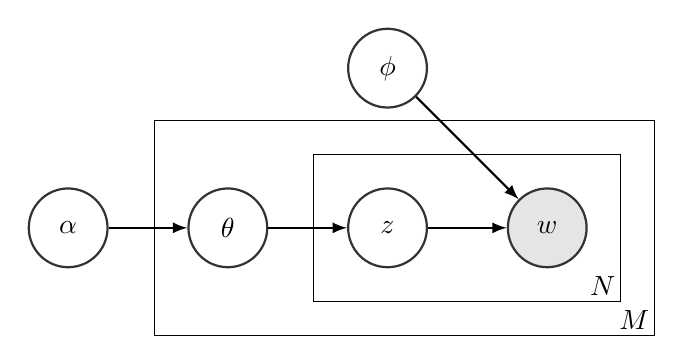
\begin{tikzpicture}
      \tikzstyle{main}=[circle, minimum size = 10mm, thick, draw =black!80, node distance = 10mm]
      \tikzstyle{observed}=[circle, minimum size = 10mm, thick, draw=black!80, node distance = 10mm, fill = black!10]
      \tikzstyle{invismain}=[circle, minimum size = 10mm, thick, draw =white!100, node distance = 10mm]
      \tikzstyle{connect}=[-latex, thick]
      \tikzstyle{box}=[rectangle, draw=black!100, inner sep=12pt]

      \node[main] (alpha) [] { $\alpha$ };
      \node[main] (theta) [right=of alpha] { $\theta$ };
      \node[main] (z) [right=of theta] { $z$ };
      \node[main] (phi) [above=of z] { $\phi$ };
      \node[observed] (w) [right=of z] { $w$ };

      \path (alpha) edge [connect] (theta)
            (theta) edge [connect] (z)
            (z) edge [connect] (w);

      \path (phi) edge [connect] (w);

      \node[box, fit=(z) (w)] (N) {};
      \node[anchor=south east, inner sep=2pt] at (N.south east) {$N$};

      \node[box, fit=(theta) (w) (N)] (M) {};
      \node[anchor=south east, inner sep=2pt] at (M.south east) {$M$};
    \end{tikzpicture}
  \end{center}
  \caption{Graphical model for LDA, as described in~\cite{Blei:2003:LDA}.}
  \label{fig:ldamodel}
\end{figure}

It is important to point out some key assumptions with this model. First,
we assume that the number of topics $K$ is a fixed quantity known in
advance, and that each $\phi_k$ is a fixed quantity to be estimated.
Furthermore, we assume that the number of unique words $V$ fixed and known
in advance (that is, the model lacks any mechanisms for generating ``new
words'').  Each word within a document is independent (encoding the
traditional ``bag of words'' assumption), and each topic proportion
$\theta_j$ is independent.

In this formulation, we can see that the joint distribution of the topic
mixtures $\Theta$, the set of topic assignments $\mathbf{Z}$, and the words
in the corpus $\mathbf{W}$ given the hyperparameter $\alpha$ and the topics
$\Phi$ is given by
\begin{equation}
  P(\mathbf{W}, \mathbf{Z}, \Theta \mid \alpha, \Phi)
  = \prod_{j=1}^M P(\theta_j \mid \alpha)
  \prod_{t=1}^{N_j} P(z_{j,t} \mid \theta_j) P(w_{j,t} \mid
  \phi_{z_{j,t}}).
  \label{eqn:fulljoint}
\end{equation}
Most works now do not actually use this original formulation, as it has a
weakness in that it does not also place a prior on the each
$\phi_k$---since this quantity is not modeled in the machinery for
inference, it must be estimated using maximum likelihood. Choosing another
Dirichlet parameterized by $\beta$ as the prior for each $\phi_k$, the
generative model becomes:

\begin{enumerate}
  \item For $i\in[1,\ldots K]$, $\phi_i \sim Dirichlet(\beta)$
  \item For $j\in[1, \ldots, M]$,
    \begin{itemize}
      \item $\theta_j \sim Dirichlet(\alpha)$
      \item For $t \in [1,\ldots, |d_j|]$
        \begin{itemize}
          \item $z_{j,t} \sim Multinomial(\theta_j)$
          \item $w_{j,t} \sim Multinomial(\phi_{z_{j,t}})$
        \end{itemize}
    \end{itemize}
\end{enumerate}
The graphic model representation for this is given in
Figure~\ref{fig:smoothed}. \citeauthor{Blei:2003:LDA} refer to this model as
``smoothed LDA'' in their work.

\begin{figure}[h]
  \begin{center}
    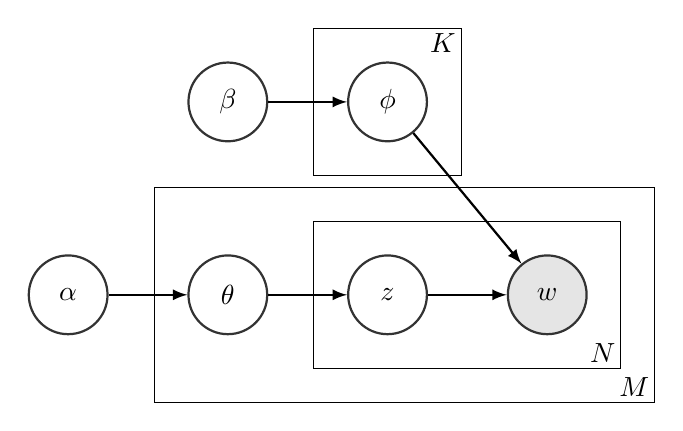
\begin{tikzpicture}
      \tikzstyle{main}=[circle, minimum size = 10mm, thick, draw =black!80, node distance = 10mm]
      \tikzstyle{observed}=[circle, minimum size = 10mm, thick, draw=black!80, node distance = 10mm, fill = black!10]
      \tikzstyle{invismain}=[circle, minimum size = 10mm, thick, draw =white!100, node distance = 10mm]
      \tikzstyle{connect}=[-latex, thick]
      \tikzstyle{box}=[rectangle, draw=black!100, inner sep=12pt]
      \tikzstyle{lbl}=[anchor=south east, inner sep=2pt];

      \node[main] (alpha) [] { $\alpha$ };
      \node[main] (theta) [right=of alpha] { $\theta$ };
      \node[main] (z) [right=of theta] { $z$ };
      \node[main] (phi) [above=of z, yshift=12pt] { $\phi$ };
      \node[main] (beta) [left=of phi] { $\beta$ };
      \node[observed] (w) [right=of z] { $w$ };

      \path (alpha) edge [connect] (theta)
            (theta) edge [connect] (z)
            (z) edge [connect] (w);

      \path (beta) edge [connect] (phi)
            (phi) edge [connect] (w);

      \node[box, fit=(z) (w)] (N) {};
      \node[lbl] at (N.south east) {$N$};

      \node[box, fit=(theta) (w) (N)] (M) {};
      \node[lbl] at (M.south east) {$M$};

      \node[box, fit=(phi)] (K) {};
      \node[anchor=north east, inner sep=2pt] at (K.north east) {$K$};
    \end{tikzpicture}
  \end{center}
  \caption{Graphical model for ``smoothed'' LDA, as described
  in \citet{Blei:2003:LDA}.}
  \label{fig:smoothed}
\end{figure}

In this ``smoothed'' formulation (which lends itself to a more fully
Bayesian inference approach), we can model the joint distribution of the
topic mixtures $\Theta$, the set of topic assignments $\mathbf{Z}$, the
words of the corpus $\mathbf{W}$, and the topics $\Phi$ by

\begin{equation}
  P(\mathbf{W}, \mathbf{Z}, \Theta, \Phi \mid \alpha, \beta)
  = \prod_{i=1}^K P(\phi_k \mid \beta) \times \prod_{j=1}^M P(\theta_j \mid
  \alpha) \prod_{t=1}^{N_j} P(z_{j,t} \mid \theta_j) P(w_{j,t} \mid
  \phi_{z_{j,t}}).
  \label{eqn:fulljointbayes}
\end{equation}
As mentioned, most approaches take the approach of
Equation~\ref{eqn:fulljointbayes}, but for the sake of completeness we will
also give the original formulation for inference for the model given by
Equation~\ref{eqn:fulljoint}.


\section{LDA vs PLSA}
Let's compare the LDA model with the PLSA model introduced by
\citet{Hofmann:1999:UAI}, as there are critical differences that motivate
all of the approximate inference algorithms for LDA.

In PLSA, we assume that the topic word distributions
$\phi_i$ and the document topic proportions $\theta_j$\footnote{These are
often called $\theta_i$ and $\pi_j$, respectively, in the standard PLSA
notation. We will use the LDA notation throughout this note.} are
\emph{parameters} in the model. By comparison, (the smoothed version of)
LDA treats each $\phi_i$ and $\theta_j$ as \emph{latent variables}. This
small difference has a dramatic impact on the way we infer the quantities
of interest in topic models. After all, the quantities we are interested in
are the distributions $\Phi$ and $\Theta$. We can use the EM algorithm to
find the maximum likelihood estimate for these quantities in PLSA, since
they are modeled as parameters. After our EM algorithm converges, we can
simply inspect the learned parameters to accomplish our goal of finding the
topics and their coverage across documents in a corpus.

In LDA, however, these quantities must be \emph{inferred} using Bayesian
inference because they themselves are \emph{latent variables}, just like
the $\mathbf{Z}$ are inferred in PLSA. Specifically, in LDA we are
interested in $P(\mathbf{Z}, \Theta, \Phi \mid \mathbf{W}, \alpha, \beta)$,
the posterior distribution of the latent variables given the parameters
$\alpha$ and $\beta$ and our observed data $\mathbf{W}$. If we write this
as
\begin{equation}
  P(\mathbf{Z}, \Theta, \Phi \mid \textbf{W}, \alpha, \beta) = \frac{P(\mathbf{W}, \mathbf{Z},
  \Theta, \Phi \mid \alpha, \beta)}{P(\mathbf{W} \mid \alpha, \beta)}.
\end{equation}
we can see that this distribution is intractable by looking at the form of
the denominator
\begin{align*}
  P(\mathbf{W} \mid \alpha, \beta)
  &=
  \int_\Phi
  \int_\Theta
  \sum_\mathbf{Z}
  P(\mathbf{W}, \mathbf{Z}, \Theta, \Phi \mid \alpha, \beta)
  d\Theta
  d\Phi\\
  &=
  \int_\Phi
  p(\Phi \mid \beta)
  \int_\Theta
  p(\Theta \mid \alpha)
  \sum_{\mathbf{Z}}
  p(\mathbf{Z} \mid \Theta)
  p(\mathbf{W} \mid \mathbf{Z}, \Phi)
  d\Theta
  d\Phi
\end{align*}
and observing the coupling between $\Theta$ and $\Phi$ in the summation
over the latent topic assignments. Thus, we are forced to turn to
approximate inference methods to compute the posterior distribution over
the latent variables we care about\footnote{If we are \emph{also}
interested in maximum likelihood estimates for the two parameter vectors
$\alpha$ and $\beta$, we can use the EM algorithm where the inference
method slots in as the computation to be performed during the E-step.
This results in an \emph{empirical Bayes} algorithm
often called \emph{variational EM}.}.

Why go through all this trouble? One of the main flaws of PLSA as pointed
out by \citet{Blei:2003:LDA} is that PLSA is not a \emph{fully generative}
model in the sense that you cannot use PLSA to create new documents, as the
topic proportion parameters are specific to each document in the corpus. To
generate a new document, we require some way to arrive at this parameter
vector for the new document, which PLSA does not provide. Thus, to adapt to
new documents, PLSA has to use a heuristic where the new document is
``folded in'' and EM is re-run (holding the old parameters fixed) to
estimate the topic proportion parameter for this new document. This is not
probabilistically well motivated. LDA, on the other hand, provides a
complete generative model for the brand new document by assuming that the
topic proportions for this document are drawn from a Dirichlet
distribution.

In practice, \citet{Lu:2011:JIR} showed PLSA and LDA tend to perform
similarly when used as a component in a downstream task (like clustering or
retrieval), with LDA having a slight advantage for document classification
due to its ``smoothed'' nature causing it to avoid overfitting. However, if
your goal is to simply discover the topics present and their coverage in a
\emph{fixed corpus}, the difference between PLSA and LDA is often
negligible.

\section{Variational Inference for LDA}
\subsection{Original (Un-smoothed) Formulation}

\citet{Blei:2003:LDA} give an inference method based on \emph{variational
inference} to approximate the posterior distribution of interest. The key
idea here is to design a family of distributions $Q$ that are tractable and
have parameters which can be tuned to approximate the desired posterior
$P$. The approach taken in the paper is often referred to as a \emph{mean
field approximation}, where they consider a family of distributions $Q$
that are fully factorized. In particular, for LDA they derive the
variational distribution as
\begin{align}
  Q(\mathbf{Z}, \Theta \mid \gamma, \pi)
  &= \prod_{j=1}^M q_j(\mathbf{z}_j, \theta_j \mid \gamma_j, \pi_j)\\
  &= \prod_{j=1}^M q_j(\theta_j \mid
  \gamma_j) \prod_{t=1}^{N_j} q_j(z_{j,t} \mid \pi_{j,t})
\end{align}
where $\gamma_j$ and $\pi_{j}$ are free variational parameters for the
variational distribution $q_j(\bullet)$ for document $j$. The graphic model
representation for this factorized variational distribution is given in
Figure~\ref{fig:factdist}.

\begin{figure}[h]
  \begin{center}
    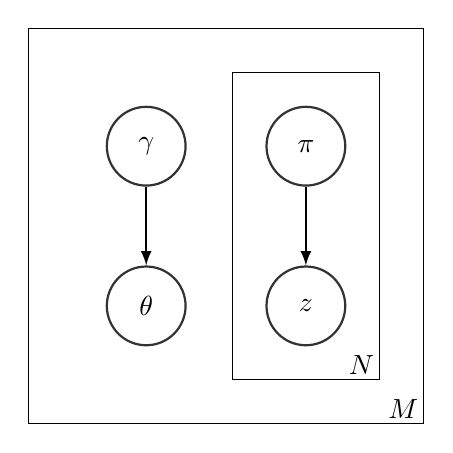
\begin{tikzpicture}
      \tikzstyle{main}=[circle, minimum size = 10mm, thick, draw =black!80, node distance = 10mm]
      \tikzstyle{observed}=[circle, minimum size = 10mm, thick, draw=black!80, node distance = 10mm, fill = black!10]
      \tikzstyle{invismain}=[circle, minimum size = 10mm, thick, draw =white!100, node distance = 10mm]
      \tikzstyle{connect}=[-latex, thick]
      \tikzstyle{box}=[rectangle, draw=black!100, inner sep=12pt]
      \tikzstyle{lbl}=[anchor=south east, inner sep=2pt];

      \node[main] (gamma) {$\gamma$};
      \node[main] (theta) [below=of gamma] {$\theta$};
      \node[main] (eta) [right=of gamma] {$\pi$};
      \node[main] (z) [below=of eta] {$z$};

      \path (gamma) edge [connect] (theta);
      \path (eta) edge [connect] (z);

      \node[box, inner sep=28pt, fit=(gamma) (theta) (eta) (z)] (M) {};
      \node[box, fit=(eta) (z)] (N) {};
      \node[lbl] at (M.south east) {$M$};
      \node[lbl] at (N.south east) {$N$};
    \end{tikzpicture}
  \end{center}
  \caption{Graphical model for the factorized variational distribution in
  \citet{Blei:2003:LDA}.}
  \label{fig:factdist}
\end{figure}

Inference is then performed by minimizing the Kullback-Leibler (KL)
divergence between the variational distributions $q_j(\bullet)$ and the
true posteriors $p(\theta_j, \mathbf{z}_j \mid \mathbf{w}_j, \alpha,
\Phi)$. If you are interested only in the algorithm, and not its
derivation, you may skip ahead to section~\ref{sec:var-inf-alg}.

\subsubsection{Variational Inference Algorithm Derivation}
\label{sec:var-inf-derivation}
Since the distribution is fully factorized across documents in both
cases, optimizing the parameters for each document in turn will optimize
the distribution as a whole, so we will focus on the document level here.

Focusing on document $j$, the KL divergence of $p$ from $q$ is

\begin{align}
  D(q \mid \mid p) &=
  \int_{\theta_j} \sum_{\mathbf{z}_j}
    q(\mathbf{z}_j, \theta_j \mid \gamma_j, \pi_j)
    \log \frac{q(\mathbf{z}_j, \theta_j \mid \gamma_j, \pi_j)}
    {p(\mathbf{z}_j, \theta_j \mid \mathbf{w}_j, \alpha, \Phi)}
  d\theta_j.
  \intertext{This can be rewritten as}
  \nonumber
  \\&=
  \int_{\theta_j} \sum_{\mathbf{z}_j}
    q(\mathbf{z}_j, \theta_j \mid \gamma_j, \pi_j)
    \log \frac{q(\mathbf{z}_j, \theta_j \mid \gamma_j, \pi_j)
    p(\mathbf{w}_j \mid \alpha, \Phi)}
    {p(\mathbf{w}_j, \mathbf{z}_j, \theta_j \mid \alpha, \Phi)}
  d\theta_j
  \nonumber
  \\&=
  \int_{\theta_j} \sum_{\mathbf{z}_j}
    q(\mathbf{z}_j, \theta_j \mid \gamma_j, \pi_j)
    \log \frac{q(\mathbf{z}_j, \theta_j \mid \gamma_j, \pi_j)}
    {p(\mathbf{w}_j, \mathbf{z}_j, \theta_j \mid \alpha, \Phi)}
  d\theta_j
  + \log p(\mathbf{w}_j \mid \alpha, \Phi).
  \nonumber
\end{align}
Noting that $\log p(\mathbf{w}_j \mid \alpha, \Phi)$ is fixed with respect
to $q$, we then want to minimize the first term in the expression
\begin{equation*}
\begin{split}
  &\int_{\theta_j} \sum_{\mathbf{z}_j}
    q(\mathbf{z}_j, \theta_j \mid \gamma_j, \pi_j)
    \log \frac{q(\mathbf{z}_j, \theta_j \mid \gamma_j, \pi_j)}
    {p(\mathbf{w}_j, \mathbf{z}_j, \theta_j \mid \alpha, \Phi)}
  d\theta_j
  \\&\quad=
  \int_{\theta_j} \sum_{\mathbf{z}_j}
    q(\mathbf{z}_j, \Theta \mid \gamma_j, \phi_j)
    \log q(\mathbf{z}_j, \Theta \mid \gamma_j, \pi_j)
  d\theta_j
  -
  \int_{\theta_j} \sum_{\mathbf{z}_j}
    q(\mathbf{z}_j, \theta_j \mid \gamma_j, \pi_j)
    \log p(\mathbf{w}_j, \mathbf{z}_j, \theta_j \mid \alpha, \Phi)
  d\theta_j
  \\&\quad=
  E_q\left[\log q(\mathbf{z}_j, \theta_j \mid \gamma_j, \pi_j)\right]
  -
  E_q\left[\log p(\mathbf{w}_j, \mathbf{z}_j, \theta_j \mid \alpha,
  \Phi)\right].
\end{split}
\end{equation*}
Thus, if we define
\begin{equation}
\begin{split}
  L(\gamma_j, \pi_j \mid \alpha, \Phi)
  &=
  E_q\left[\log p(\mathbf{w}_j, \mathbf{z}_j, \theta_j \mid \alpha, \Phi)\right]
  - E_q\left[\log q(\mathbf{z}_j, \Theta \mid \gamma_j, \pi_j)\right]
  \\&=
  E_q\left[\log p(\theta_j \mid \alpha)\right]
  + E_q\left[\log p(\mathbf{z}_j \mid \theta_j)\right]
  + E_q\left[\log p(\mathbf{w}_j \mid \mathbf{z}_j, \Phi)\right]
  \\&\quad
  - E_q\left[\log q(\theta_j \mid \gamma_j)\right]
  - E_q\left[\log q(\mathbf{z}_j \mid \pi_j)\right]
\end{split}
\end{equation}
then we can see that maximizing $L(\bullet)$ will minimize $D(q\mid\mid
p)$. Proceeding to simplify each of the expectations in $L(\bullet)$, we
first have
\begin{align}
  E_q\left[\log p(\theta_j \mid \alpha)\right]
  &=
  E_q\left[
    \log \left(
      \frac{\Gamma(\sum_{i=1}^K \alpha_i)}
      {\prod_{i=1}^K \Gamma(\alpha_i)}
      \prod_{i=1}^K \theta_{j,i}^{\alpha_i - 1}
    \right)
  \right]
  \\&=
  E_q\left[
    \log \Gamma\left(\sum_{i=1}^K \alpha_i\right)
    - \sum_{i=1}^k \log \Gamma(\alpha_i)
    + \sum_{i=1}^k (\alpha_i - 1)\log \theta_{j,i}
  \right]
  \\&=
  \log \Gamma\left(\sum_{i=1}^K \alpha_i\right)
  - \sum_{i=1}^k \log \Gamma(\alpha_i)
  + \sum_{i=1}^k (\alpha_i - 1)E_q\left[\log \theta_{j,i}\right].
\end{align}
We're left with a single expectation $E_q[\log \theta_{j,i}]$. We can now
use the fact that $\theta_j \sim Dirichlet(\gamma_j)$, which is a member of
the exponential family (see
Equation~\ref{eqn:dirichlet-as-exponential-family}), to solve for this
expectation. Recall that the sufficient statistic for the above Dirichlet
is $\log \theta_{j,i}$ and that it has a log normalizer of
\begin{equation}
  a(\gamma_j) = \sum_{i=1}^k \log
  \Gamma(\gamma_{j,i}) - \log \Gamma\left(\sum_{i=1} \gamma_{j,i}\right).
\end{equation}
Thus,
\begin{align}
  \label{eqn:digamma-beg}
  E_q\left[\log \theta_{j,i}\right]
  &=
  \frac{d}{d\gamma_{j,i}} a(\gamma_j)
  \\&=
  \frac{d}{d\gamma_{j,i}} \sum_{k=1}^K \log \Gamma(\gamma_{j,k})
  - \log \Gamma\left(\sum_{l=1}^K \gamma_{j,l}\right)
  \\&=
  \Psi(\gamma_{j,i}) - \Psi\left(\sum_{l=1}^K \gamma_{j,l}\right)
  \label{eqn:digamma-end}
\end{align}
where $\Psi(\bullet)$ is the ``digamma'' function, the first derivative of
the log Gamma function. Plugging this in, we arrive at
\begin{equation}
  E_q\left[\log p(\theta_j \mid \alpha)\right]
  =
  \log \Gamma\left(\sum_{i=1}^K \alpha_i\right)
  - \sum_{i=1}^k \log \Gamma(\alpha_i)
  + \sum_{i=1}^k (\alpha_i - 1)
  \left(\Psi(\gamma_{j,i}) - \Psi\left(\sum_{l=1}^K \gamma_{j,l}\right)\right)
\end{equation}
Next, we turn our attention to the second term of $L(\bullet)$. Let
$\mathbb{1}(\bullet)$ be an indicator function equal to 1 if the condition
is true. Then, we have
\begin{align}
  E_q\left[\log p(z_j \mid \theta_j)\right]
  &=
  E_q\left[\sum_{t=1}^{N_j} \sum_{i=1}^K \mathbb{1}(z_{j,t} = i)\log
  \theta_{j,i}\right]
  \\&=
  \sum_{t=1}^{N_j} \sum_{i=1}^K E_q[\mathbb{1}(z_{j,t} = i)]E_q[\log
  \theta_{j,i}]
  \\&=
  \sum_{t=1}^{N_j} \sum_{i=1}^K \pi_{j,t,i}
  \left(\Psi(\gamma_{j,i}) - \Psi\left(\sum_{l=1}^K \gamma_{j,l}\right)\right),
\end{align}
where we have again used
equations~\ref{eqn:digamma-beg}--\ref{eqn:digamma-end} for simplifying
$E_q[\log \theta_{j,i}]$. The third term can be simplified as follows:
\begin{align}
  E_q\left[\log p(w_i \mid z_j, \Phi)\right]
  &=
  E_q\left[
    \sum_{t=1}^{N_j} \sum_{i=1}^K \sum_{r=1}^V
    \mathbb{1}(z_{j,t} = i)\mathbb{1}(w_{j,t} = r)\log \phi_{i,r}
  \right]
  \\&=
  \sum_{t=1}^{N_j} \sum_{i=1}^K \sum_{r=1}^V
  E_q[\mathbb{1}(z_{j,t} = i)
  \mathbb{1}(w_{j,t} = r)
  \log \phi_{i,r}]
  \\&=
  \sum_{t=1}^{N_j} \sum_{i=1}^K \sum_{r=1}^V
  \pi_{j,t,i} \mathbb{1}(w_{j,t} = r) \log \phi_{i,r}.
\end{align}
The fourth term is very similar to the first, and is
\begin{equation}
  E_q\left[\log q(\theta_j \mid \gamma_j) \right]
  =
  \log \Gamma\left(\sum_{i=1}^K \gamma_{j,i}\right)
  - \sum_{i=1}^K \log \Gamma(\gamma_{j,i})
  + \sum_{i=1}^K (\gamma_{j,i} - 1)
  \left(\Psi(\gamma_{j,i}) - \Psi\left(\sum_{l=1}^K \gamma_{j,l}\right)\right)
\end{equation}
The fifth and final term can be reduced as
\begin{align}
  E_q\left[\log q(z_j \mid \pi_j)\right]
  &=
  E_q\left[
    \sum_{t=1}^{N_j} \sum_{i=1}^K
    \mathbb{1}(z_{j,t} = i) \log \pi_{j,t,i}
  \right]
  \\&=
  \sum_{t=1}^{N_j} \sum_{i=1}^K
  E_q[\mathbb{1}(z_{j,t} = i)] \log \pi_{j,t,i}
  \\&=
  \sum_{t=1}^{N_j} \sum_{i=1}^K
  \pi_{j,t,i} \log \pi_{j,t,i},
\end{align}
and thus we arrive at
\begin{equation}
  \begin{split}
    L(\gamma_j, \pi_j \mid \alpha, \Phi)
    &=
    \log \Gamma\left(\sum_{i=1}^K \alpha_i\right)
    - \sum_{i=1}^k \log \Gamma(\alpha_i)
    + \sum_{i=1}^k (\alpha_i - 1)
    \left(\Psi(\gamma_{j,i}) - \Psi\left(\sum_{l=1}^K \gamma_{j,l}\right)\right)
    \\&+
    \sum_{t=1}^{N_j} \sum_{i=1}^K \pi_{j,t,i}
    \left(\Psi(\gamma_{j,i}) - \Psi\left(\sum_{l=1}^K \gamma_{j,l}\right)\right)
    \\&+
    \sum_{t=1}^{N_j} \sum_{i=1}^K \sum_{r=1}^V
    \pi_{j,t,i} \mathbb{1}(w_{j,t} = r) \log \phi_{i,r}
    \\&-
    \log \Gamma\left(\sum_{i=1}^K \gamma_{j,i}\right)
    + \sum_{i=1}^K \log \Gamma(\gamma_{j,i})
    - \sum_{i=1}^K (\gamma_{j,i} - 1)
    \left(\Psi(\gamma_{j,i}) - \Psi\left(\sum_{l=1}^K \gamma_{j,l}\right)\right)
    \\&-
    \sum_{t=1}^{N_j} \sum_{i=1}^K
    \pi_{j,t,i} \log \pi_{j,t,i}.
  \end{split}
\end{equation}

We can now perform a constrained maximization of $L(\bullet)$ by isolating
terms and introducing Lagrange multipliers. We start by isolating the
terms containing a single $\pi_{j,t,i}$. Noting the constraint here is
$\sum_{l = 1}^K \pi_{j,t,l} = 1$, we have
\begin{equation}
  L_{[\pi_{j,t,i}]}
  =
  \pi_{j,t,i}\left(
    \Psi(\gamma_{j,i}) - \Psi\left(\sum_{l=1}^K \gamma_{j,l}\right)
  \right)
  +
  \pi_{j,t,i} \log \phi_{i,w_{j,t}}
  -
  \pi_{j,t,i} \log \pi_{j,t,i}
  +
  \lambda \left(\sum_{l=1}^K \pi_{j,t,l} - 1\right)
\end{equation}
Taking derivatives with respect to $\pi_{j,t,l}$, we have
\begin{equation}
  \frac{\partial L}{\partial \pi_{j,t,i}}
  = \Psi(\gamma_{j,i}) - \Psi\left(\sum_{l=1}^K \gamma_{j,l}\right)
  + \log \phi_{i,w_{j,t}}
  - \log \pi_{j,t,i} - 1
  + \lambda.
\end{equation}
Setting this equation to zero and solving for $\pi_{j,t,i}$, we arrive at
the update
\begin{equation}
  \pi_{j,t,i}
  \propto
  \phi_{i,w_{j,t}}
  \exp\left\{
    \Psi(\gamma_{j,i}) - \Psi\left(\sum_{l=1}^K \gamma_{j,i}\right)
  \right\}
\end{equation}
Concerning ourselves now with $\gamma_{j,i}$, which is unconstrained, we have
\begin{equation}
  \begin{split}
    L_{[\gamma_j]}
    &=
    \sum_{i=1}^k (\alpha_i - 1)
    \left(\Psi(\gamma_{j,i}) - \Psi\left(\sum_{l=1}^K \gamma_{j,l}\right)\right)
    \\&+
    \sum_{t=1}^{N_j} \sum_{i=1}^K \pi_{j,t,i}
    \left(\Psi(\gamma_{j,i}) - \Psi\left(\sum_{l=1}^K \gamma_{j,l}\right)\right)
    \\&-
    \log \Gamma\left(\sum_{i=1}^K \gamma_{j,i}\right)
    + \sum_{i=1}^K \log \Gamma(\gamma_{j,i})
    - \sum_{i=1}^K (\gamma_{j,i} - 1)
    \left(\Psi(\gamma_{j,i}) - \Psi\left(\sum_{l=1}^K
    \gamma_{j,l}\right)\right),
  \end{split}
\end{equation}
which can be simplified to
\begin{equation}
  L_{[\gamma_j]}
  =
  \sum_{i=1}^K \left(\alpha_i + \sum_{t=1}^{N_j} \pi_{j,t,i} -
    \gamma_{j,i}\right)
  \left(
    \Psi(\gamma_{j,i}) - \Psi\left(\sum_{l=1}^K \gamma_{j,l}\right)
  \right)
  - \log \Gamma\left(\sum_{l=1}^K \gamma_{j,l}\right)
  + \sum_{i=1}^K \log \Gamma(\gamma_{j,i})
\end{equation}
Deriving with respect to $\gamma_{j,i}$, we get
\begin{align*}
  \frac{\partial L}{\partial \gamma_{j,i}}
  &=
  \frac{\partial}{\partial \gamma_{j,i}}
  \sum_{l=1}^K \left(\alpha_l + \sum_{t=1}^{N_j} \pi_{j,t,l} -
    \gamma_{j,l}\right)
  \Psi(\gamma_{j,l})
  -
  \sum_{l=1}^K \left(\alpha_l + \sum_{t=1}^{N_j} \pi_{j,t,l} -
    \gamma_{j,l}\right)
  \Psi(\sum_{l=1}^K \gamma_{j,l})
  \\&\quad-
  \log \Gamma\left(\sum_{l=1}^K \gamma_{j,l}\right)
  +
  \sum_{l=1}^K \log \Gamma\left(\gamma_{j,l}\right)
  \\&=
  -\Psi(\gamma_{j,i}) + \Psi'(\gamma_{j,i})\left(\alpha_i + \sum_{t=1}^{N_j}
  \pi_{j,t,i} - \gamma_{j,i}\right)
  \\&\quad+
  \Psi\left(\sum_{l=1}^K \gamma_{j,l}\right)
  - \Psi'\left(\sum_{l=1}^K \gamma_{j,l}\right)\sum_{l=1}^K \left(
    \alpha_l + \sum_{t=1}^{N_j} \pi_{j,t,i} - \gamma_{j,l}
  \right)
  \\&\quad-
  \Psi\left(\sum_{l=1}^K \gamma_{j,l} \right)
  + \Psi(\gamma_{j,i})
  \\&=
  \Psi'(\gamma_{j,i})\left(
    \alpha_i + \sum_{t=1}^{N_j} \pi_{j,t,i} - \gamma_{j,i}
  \right)
  - \Psi'\left(\sum_{l=1}^K \gamma_{j,l}\right)\sum_{l=1}^K \left(
    \alpha_l + \sum_{t=1}^{N_j} \pi_{j,t,i} - \gamma_{j,l}
  \right).
\end{align*}
Setting this equal to zero and taking the obvious solution, we arrive at
\begin{equation}
  \gamma_{j,i} = \alpha_i + \sum_{t=1}^{N_j} \pi_{j,t,i}.
\end{equation}

\subsubsection{Variational Inference Algorithm}
\label{sec:var-inf-alg}

The following updates have been derived to minimize the KL divergence from
$p$ to $q$ for each document $j$:
\begin{align}
  \pi_{j,t,i} &\propto \phi_{i,w_{j,t}} \exp\left(\Psi(\gamma_{j,i}) -
  \Psi\left(\sum_{k=1}^K \gamma_{j,k}\right)\right)\\
  \gamma_{j,i} &= \alpha_i + \sum_{t=1}^{N_j} \pi_{j,t,i}.
\end{align}
where $\Psi(\bullet)$ is the ``digamma'' function. It is important to note
here that this inference process is done on a per-document level (hence the
subscript $j$ in all of these parameters). The authors speculate that the
number of iterations required is linear in the length of the document
($N_j$), and the number of operations within the method is $O(Nk)$---thus
they arrive at the running time estimate $O(N_j^2 k)$. However, since this
procedure would need to be run for every document $j$, the full running
time is multiplied by another factor of $M$.

While the procedure's found parameters $\gamma_j$ can be used in place of
the model's latent variables $\theta_j$, it has no provision for directly
finding the model parameters $\Phi$, the actual topics. The authors propose
a \emph{variational expectation maximization} (variational EM) for
estimating this parameter. The essential idea is this: run the previously
described variational inference method for each document $j$ until
convergence. Then, using these fixed variational parameters, update the
estimates for the model parameter $\Phi$ given these fixed variational
parameters. These two steps are done iteratively until the lower bound on
the log likelihood converges.

Specifically, the variational EM algorithm derived is the following:
\begin{description}
  \item[E-step:]
    Minimize $KL(q \mid\mid p)$ by performing the following updates until
    convergence:
    \begin{align*}
      \pi_{j,t,i} &\propto
      \phi_{i,w_{j,t}} \exp \left(
        \psi(\gamma_{j,i}) - \psi\left(\sum_{k=1}^K \gamma_{j,k}\right)
      \right)\\
      \gamma_{j,i} &= \alpha_i + \sum_{t=1}^{N_j} \pi_{j,t,i}.
    \end{align*}

    $q$ now is a good approximation to the posterior distribution $p$.
  \item[M-step:] Using $q$, re-estimate the parameters $\Phi$.
    Specifically, since $\pi_{j,t,i}$ represents the probability that word
    $w_{j,t}$ was assigned to topic $i$, we can compute and re-normalize
    expected counts:
    \begin{equation}
        \phi_{i,v} \propto \sum_{j=1}^M
        \sum_{t=1}^{N_j} \pi_{j,t,i} \mathbb{1}(w_{j,t} = v)
        \label{eqn:varemphi}
    \end{equation}
    where $\mathbb{1}(\bullet)$ is the indicator function that takes value
    1 if the condition is true, and value 0 otherwise.
\end{description}

\subsection{Smoothed Formulation}

In their smoothed formulation (see Figure~\ref{fig:smoothed}),
\citet{Blei:2003:LDA} find a factorized distribution which also contains
$\Phi$ as a random variable with a Dirichlet prior with hyperparameter
$\beta$ as

\begin{equation}
  Q(\Phi, \mathbf{Z}, \Theta \mid \lambda, \pi, \gamma) =
  \prod_{i=1}^K Dir(\phi_i \mid \lambda_i) \prod_{j=1}^M q_j(\theta_j,
  \mathbf{z}_j \mid \pi_j, \gamma_j)
\end{equation}

The graphic model for this variational distribution is given in
Figure~\ref{fig:factdistsmooth}.

\begin{figure}[h]
  \begin{center}
    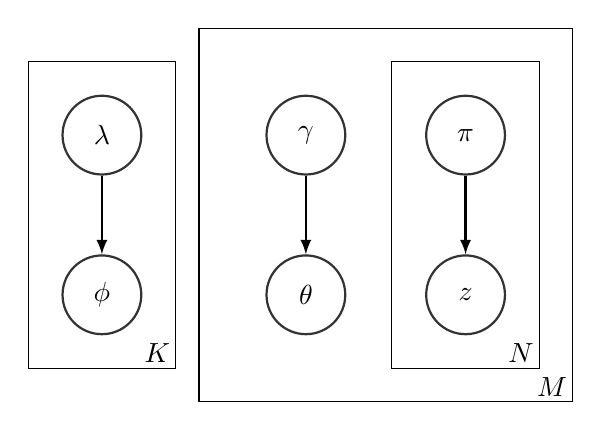
\begin{tikzpicture}
      \tikzstyle{main}=[circle, minimum size = 10mm, thick, draw =black!80, node distance = 10mm]
      \tikzstyle{observed}=[circle, minimum size = 10mm, thick, draw=black!80, node distance = 10mm, fill = black!10]
      \tikzstyle{invismain}=[circle, minimum size = 10mm, thick, draw =white!100, node distance = 10mm]
      \tikzstyle{connect}=[-latex, thick]
      \tikzstyle{box}=[rectangle, draw=black!100, inner sep=12pt]
      \tikzstyle{lbl}=[anchor=south east, inner sep=2pt];

      \node[main] (gamma) {$\gamma$};
      \node[main] (theta) [below=of gamma] {$\theta$};
      \node[main] (eta) [right=of gamma] {$\pi$};
      \node[main] (z) [below=of eta] {$z$};
      \node[main] (lambda) [left=of gamma, xshift=-16pt] {$\lambda$};
      \node[main] (phi) [below=of lambda] {$\phi$};

      \path (gamma) edge [connect] (theta);
      \path (eta) edge [connect] (z);
      \path (lambda) edge [connect] (phi);

      \node[box, inner sep=24pt, fit=(gamma) (theta) (eta) (z)] (M) {};
      \node[box, fit=(eta) (z)] (N) {};
      \node[box, fit=(lambda) (phi)] (K) {};
      \node[lbl] at (M.south east) {$M$};
      \node[lbl] at (N.south east) {$N$};
      \node[lbl] at (K.south east) {$K$};
    \end{tikzpicture}
  \end{center}
  \caption{Graphical model for the factorized variational distribution for
    ``smoothed LDA''~\cite{Blei:2003:LDA}.}
  \label{fig:factdistsmooth}
\end{figure}

The updating equations for $\gamma$ and $\pi$ remain the same as in the
previous formulation, but they add an additional update for the new
variational parameters $\lambda$ as
\begin{equation}
  \lambda_{i,v} = \beta_v + \sum_{j=1}^M \sum_{t=1}^{N_j} \pi_{j,t,v}
  \mathbb{1}(w_{j,t} = v).
\end{equation}
This bears a striking resemblance to the update for $\phi_{i,v}$ in the
variational EM algorithm given in the previous section's
Equation~\ref{eqn:varemphi}, but with the addition of the prior's
pseudo-counts $\beta_v$.

It is worth noting that now that the distributions of interest $\Phi$ and
$\Theta$ are both latent variables, the inference process itself will
generate all of the distributions we are interested in, so we do not have
to run the inference algorithm in a loop to re-estimate the values for
$\Phi$ as we did before. We may choose to run an EM algorithm to learn the
parameters $\alpha$ and $\beta$, but this is not explored in this note.

\subsection{Evaluation and Implementation Concerns}

The inference method proposed for the original model consists of solving an
optimization problem for every document to find the variational parameters
$\gamma_j$ and $\pi_{j,t} \forall j\in[1,\ldots,N_j]$, then the results of
these $M$ optimization problems to update the model parameters
$\phi_i\forall i\in[1,\ldots,K]$. Major criticisms of this method are not
just limited to the fact that it does not treat $\Phi$ as a random
variable---it also contains many calls to the $\Psi(\bullet)$ function
which is known to hurt performance. Further, the memory requirements for
variational inference are larger than some of the alternative methods, but
this method has the advantage of being deterministic (where many
alternatives are probabilistic).

Other arguments (such as the ones presented in \citet{Teh:2007:CVB})
criticize the method based on its inaccuracy: the strong independence
assumption introduced in the fully factorized variational distribution
eliminates the strong dependence between the latent variables $\mathbf{Z}$,
$\Theta$, and $\Phi$ which can lead to inaccurate estimates of the
posterior due to the loose upper bound on the negative log likelihood.

\section{Collapsed Gibbs Sampling for LDA}

Another general approach for posterior inference with intractable
distributions is to appeal to Markov-chain Monte Carlo methods. Gibbs
sampling is one such algorithm, but there are many others (such as
Metropolis Hastings). Here, the goal is to produce samples from a
distribution that is hard to sample from directly. The Gibbs sampling
method is applicable when the distribution to sample from is intractable,
but the \emph{conditional distribution} of a specific variable \emph{given
all the others} can be computed easily. The algorithm proceeds in
``rounds'' (sometimes called ``epochs'') where each latent variable is
sampled in turn conditioned on the current values of all of the other
latent variables. This process ``sweeps'' through all of the latent
variables and the round ends when all of the latent variables have been
re-sampled according to their full conditional distributions. This strategy
can be shown to eventually (after some amount of burn-in time) result in
accurate samples from the true posterior distribution.

In the case of LDA, we can make a further simplification that will enable
the sampler to converge faster. Because the priors over $\Phi$ and $\Theta$
are \emph{conjugate}, they can be \emph{integrated out} of the joint
distribution, resulting in a distribution $P(\mathbf{W}, \mathbf{Z} \mid
\alpha, \beta)$, which we can then use to build a Gibbs sampler over
$\mathbf{Z}$. This process of integrating out the conjugate priors is often
called ``collapsing'' the priors, and thus a sampler built in this way is
often called a ``collapsed Gibbs sampler''. In this section, we will show
how to derive a collapsed Gibbs sampler for LDA and also introduce a
variation of the algorithm that, while approximate, can leverage parallel
computation resources (either on a single system with multiple threads or
multiple systems).

These methods are generally attractive in the sense that they are typically
easily implemented, and the sampling method itself has nice guarantees
about convergence to the true posterior. Unfortunately, because it is a
randomized algorithm, it does not have the deterministic guarantees that
the previous variational inference method does.


\label{sec:cgs}
\subsection{Original Method}
The general idea behind Gibbs sampling methods is to take repeated samples
from the \emph{full conditional} distribution for each latent variable in
turn, iteratively. In this way, the current assignments for all other
latent variables influence the sampling for the ``replacement'' latent
variable in the current iteration.

One could in theory apply Gibbs sampling directly to LDA, but this would
exhibit slow mixing due to the interactions between the latent variables.
Instead, \citet{Griffiths:2004:Topics} derive a sampler that integrates out
the variables $\Theta$ and $\Phi$ by taking advantage of the fact that the
Dirichlet is the conjugate prior of the multinomial in order to simplify
the integrals. Then, based on the posterior distribution of the latent
topic assignments $\mathbf{Z}$, we can get estimates for the distributions
$\Theta$ and $\Phi$.

The key observation is this: suppose that we have the joint distribution of
the corpus and the topic assignments $P(\mathbf{W}, \mathbf{Z} \mid \alpha,
\beta)$ with the parameters $\Theta$ and $\Phi$ integrated out. Then,
because $\mathbf{W}$ is observed, we simply need to sample each $z_{m,n}$
in turn, given the full conditional consisting of all other topic
assignments $\mathbf{Z}_{\neg m,n}$. We can see that

\begin{align}
  P(z_{m,n} = k \mid \mathbf{Z}_{\neg m,n}, \mathbf{W}, \alpha, \beta)
  &=
  \frac{P(z_{m,n} = k, \mathbf{Z}_{\neg m,n}, \mathbf{W} \mid \alpha, \beta)}
  {P(\mathbf{Z}_{\neg m,n}, \mathbf{W} \mid \alpha, \beta)}\nonumber\\
  \label{eqn:full-conditional}
  & \propto P(z_{m,n} = k, \mathbf{Z}_{\neg m,n}, \mathbf{W} \mid \alpha,
    \beta)
\end{align}

Thus, with just a definition of $P(\mathbf{W}, \mathbf{Z} \mid \alpha,
\beta)$, we can derive a Gibbs sampler that iterates over the topic
assignments $z_{j,t}$. One can find this distribution by performing the
integration over $\Theta$ and $\Phi$, which we will show in the next
section.

\subsection{Integrating Out the Priors in LDA}

We start by noting that
\begin{align}
  P(\mathbf{W}, \mathbf{Z} \mid \alpha, \beta)
  &= P(\mathbf{Z} \mid \alpha, \beta)P(\mathbf{W} \mid \mathbf{Z}, \alpha,
  \beta)
  \intertext{by the definition of conditional probability, and}
  &= P(\mathbf{Z} \mid \alpha)P(\mathbf{W} \mid \mathbf{Z}, \beta)
\end{align}
according to our modeling assumptions. We can now focus on these two terms
individually.

Starting with $P(\mathbf{Z} \mid \alpha)$, we have that
\begin{equation}
  P(\mathbf{Z} \mid \alpha)
  &= \int P(\Theta \mid \alpha) P(\mathbf{Z} \mid \Theta) d\Theta
\end{equation}
from our model definition. Focusing on the prior term $P(\Theta \mid
\alpha)$, we have
\begin{equation}
  P(\Theta \mid \alpha)
  = \prod_{j=1}^M P(\theta_j \mid \alpha)
  = \prod_{j=1}^M \frac{1}{B(\alpha)} \prod_{i=1}^K \theta_{j,i}^{\alpha_i
  - 1}.
\end{equation}
We also know that
\begin{equation}
  P(\mathbf{Z} \mid \Theta) = \prod_{j=1}^M \prod_{t=1}^{N_j}
  \theta_{j,z_{j,t}} = \prod_{j=1}^M \prod_{i=1}^K
  \theta_{j,i}^{\sigma_{j,i}}
\end{equation}
where
\begin{equation}
  \sigma_{j,k} = \sum_{t=1}^{N_j} \mathbb{1}(z_{j,t} = k)
\end{equation}
is the number of times we observe topic $k$ in document $j$. Combining
these two distributions, we can see that
\begin{align}
  \int P(\Theta \mid \alpha) P(\mathbf{Z} \mid \Theta) d\Theta
  &= \prod_{j=1}^M \int \frac{1}{B(\alpha)} \prod_{i=1}^K
  \theta_{j,i}^{\sigma_{j,i} + \alpha_i - 1} d\theta_j\\
  &= \prod_{j=1}^M \frac{1}{B(\alpha)}
  \int \prod_{i=1}^K \theta_{j,i}^{\sigma_{j,i} + \alpha_i - 1} d\theta_j.
  \intertext{We can now apply the property we derived in
  Equation~\ref{eqn:integral-beta-property} to show that}
  P(\mathbf{Z} \mid \alpha)
  &= \prod_{j=1}^M \frac{B(\alpha + \sigma_j)}{B(\alpha)},
\end{align}
where $\sigma_j$ is the count vector over topics in document $j$.

Turning our attention to $P(\mathbf{W} \mid \mathbf{Z}, \beta)$, we see a
similar story. Namely
\begin{equation}
  P(\mathbf{W} \mid \mathbf{Z}, \beta)
  = \int P(\Phi \mid \beta) P(\mathbf{W} \mid \mathbf{Z}, \Phi) d\Phi.
\end{equation}
We also know that
\begin{equation}
  P(\Phi \mid \beta) = \prod_{i=1}^K P(\phi_i \mid \beta)
  = \prod_{i=1}^K \frac{1}{B(\beta)} \prod_{r=1}^V
  \phi_{i,r}^{\beta_r - 1},
\end{equation}
and
\begin{equation}
  P(\mathbf{W} \mid \mathbf{Z}, \Phi)
  = \prod_{j=1}^M \prod_{t=1}^{N_j} P(w_{j,t} \mid \phi_{z_{j,t}})
  = \prod_{i=1}^K \prod_{r=1}^V \phi_{i,r}^{\delta_{i,r}},
\end{equation}
where $\delta_{i,r}$ is defined analogously to $\sigma_{j,k}$ as the number
of times word type $r$ appears in topic $i$. Thus,
\begin{align}
  \int P(\phi \mid \beta)P(\mathbf{W} \mid \mathbf{Z}, \Phi) d\Phi
  &= \prod_{i=1}^K \int \frac{1}{B(\beta)} \prod_{r=1}^V
  \phi_{i,r}^{\delta_{i,r} + \beta_r - 1} d\phi_i\\
  &= \prod_{i=1}^K \frac{1}{B(\beta)} \int \prod_{r=1}^V
  \phi_{i,r}^{\delta_{i,r} + \beta_r - 1} d\phi_i.
\end{align}
We can again apply the property we derived in
Equation~\ref{eqn:integral-beta-property} to show that
\begin{equation}
  P(\mathbf{W} \mid \mathbf{Z}, \beta)
  =
  \prod_{i=1}^K \frac{B(\beta + \delta_i)}{B(\beta)}
\end{equation}
where $\delta_i$ is the count vector associated with topic $i$. This leads
to a \emph{collapsed} joint probability definition of
\begin{equation}
  P(\mathbf{W}, \mathbf{Z} \mid \alpha, \beta)
  = \left(
    \prod_{j=1}^M \frac{B(\alpha + \sigma_j)}{B(\alpha)}
  \right)
  \left(
    \prod_{i=1}^K \frac{B(\beta + \delta_i)}{B(\beta)}
  \right).
\end{equation}

\subsection{Deriving the Collapsed Gibbs Sampler}
We showed in the previous section that we can integrate out the priors over
$\Phi$ and $\Theta$ and arrive at
\begin{align}
  P(\mathbf{W}, \mathbf{Z} \mid \alpha, \beta)
  &= \int_\Theta
     \int_\Phi
     \prod_{i=1}^K P(\phi_i \mid \beta)
     \prod_{j=1}^M P(\theta_j \mid \alpha)
     \prod_{t=1}^{N_j} P(z_{j,t} \mid \theta_j)
     P(w_{j,t} \mid \phi_{z_{j,t}}) d\Theta d\Phi\nonumber\\
  &=\left(
    \prod_{j=1}^M \frac{B(\alpha + \sigma_j)}{B(\alpha)}
  \right)
  \left(
    \prod_{i=1}^K \frac{B(\beta + \delta_i)}{B(\beta)}
  \right)\\
  &= \left(
       \frac{\Gamma\left(\sum_{i=1}^K \alpha_i\right)}
       {\prod_{i=1}^K \Gamma(\alpha_i)}
     \right)^M
     \prod_{j=1}^M
     \frac{\prod_{i=1}^K \Gamma(\sigma_{j,i} + \alpha_i)}
     {\Gamma\left(\sum_{i=1}^K\sigma_{j,i} + \alpha_i\right)}\nonumber\\
     &\quad\;\times
     \left(
       \frac{\Gamma\left(\sum_{r=1}^V \beta_r\right)}
       {\prod_{r=1}^V \Gamma(\beta_r)}
     \right)^K
     \prod_{i=1}^K
     \frac{\prod_{r=1}^V \Gamma(\delta_{i,r} + \beta_r)}
     {\Gamma\left(\sum_{r=1}^V \delta_{i,r} + \beta_r\right)}
\end{align}
where $\sigma_{j,i}$ is the number of times topic $i$ has been chosen for
words in document $j$, and $\delta_{i,r}$ is the number of times topic $i$
has been chosen for word type $r$. We can now derive the sampler on the
basis of Equation~\ref{eqn:full-conditional}.

We start by dropping the two coefficients in front of the product over the
documents and the product over the topics by noting that these do not
depend on the specific topic assignment $z_{m,n}$. We then have that
\begin{align}
  P(\mathbf{W}, z_{m,n} = k, \mathbf{Z}_{\neg m,n} \mid \alpha, \beta)
  &\propto
  \prod_{j=1}^M
   \frac{\prod_{i=1}^K \Gamma(\sigma_{j,i} + \alpha_i)}
   {\Gamma\left(\sum_{i=1}^K\sigma_{j,i} + \alpha_i\right)}
   \times
   \prod_{i=1}^K
     \frac{\prod_{r=1}^V \Gamma(\delta_{i,r} + \beta_r)}
     {\Gamma\left(\sum_{r=1}^V \delta_{i,r} + \beta_r\right)}.
  \intertext{Now we can extract only those terms that depend on the
  the position $(m, n)$ we are sampling for (as all others are constants as
  we vary $z_{m,n}$):}
  &\label{eqn:full-conditional-only-mn}
  \propto
  \frac{\prod_{i=1}^K \Gamma(\sigma_{m,i} + \alpha_i)}
  {\Gamma\left(\sum_{i=1}^K \sigma_{m,i} + \alpha_i\right)}
  \times
  \prod_{i=1}^K
  \frac{\Gamma(\delta_{i,w_{m,n}} + \beta_{w_{m,n}})}
  {\Gamma\left(\sum_{r=1}^V \delta_{i,r} + \beta_r\right)}
\end{align}

Now let's let
\begin{equation}
  \sigma_{j,i}^{\neg m,n} = \begin{cases}
    \sigma_{j,i} - 1 & \text{if } j = m \text{ and } i = z_{m,n}\\
    \sigma_{j,i} & \text{otherwise}
  \end{cases}
\end{equation}
be the number of times we see topic $i$ in document $j$, but excluding the
current assignment $z_{m,n}$. Similarly, let
\begin{equation}
  \delta_{i,r}^{\neg m,n} = \begin{cases}
    \delta_{i,r} - 1 & \text{if } i = z_{m,n} \text{ and } r = w_{m,n}\\
    \delta_{i,r} & \text{otherwise}.
  \end{cases}
\end{equation}
We can then rewrite the right hand side of
Equation~\ref{eqn:full-conditional-only-mn} above as
\begin{multline}
  \frac{\left(\prod_{i=1; i \neq k}^K \Gamma(\sigma_{m,i}^{\neg m,n} +
  \alpha_i)\right) \Gamma(1 + \sigma_{m,k}^{\neg m,n} + \alpha_k)}
  {\Gamma\left(1 + \sum_{i=1}^K \sigma_{m,i}^{\neg m,n} + \alpha_i\right)}
  \\
  \label{eqn:extracted-products}
  \times
  \prod_{i=1; i \neq k}^K
  \frac{\Gamma(\delta_{i,w_{m,n}}^{\neg m, n} + \beta_{w_{m,n}})}
  {\Gamma\left(\sum_{r=1}^V \delta_{i,r}^{\neg m, n} + \beta_{r}\right)}
  \times
  \frac{\Gamma(1 + \delta_{k,w_{m,n}}^{\neg m, n} + \beta_{w_{m,n}})}
  {\Gamma\left(1 + \sum_{r=1}^V \delta_{k,r}^{\neg m, n} + \beta_r\right)}.
\end{multline}
Now, we use the property of the gamma function that
\begin{equation}
  \Gamma(1 + x) = x \Gamma(x)
\end{equation}
to rewrite the terms in Equation~\ref{eqn:extracted-products}, which then
becomes
\begin{multline}
  \frac{\left(\prod_{i=1; i \neq k}^K \Gamma(\sigma_{m,i}^{\neg m,n} +
  \alpha_i)\right)
  \Gamma(\sigma_{m,k}^{\neg m,n} + \alpha_k)(\sigma_{m,k}^{\neg m,n} +
  \alpha_k)}
  {\Gamma\left(\sum_{i=1}^K \sigma_{m,i}^{\neg m,n} + \alpha_i\right)
  \left(\sum_{i=1}^K \sigma_{m,i}^{\neg m,n} + \alpha_i\right)}
  \\
  \times
  \prod_{i=1; i \neq k}^K
  \frac{\Gamma(\delta_{i,w_{m,n}}^{\neg m, n} + \beta_{w_{m,n}})}
  {\Gamma\left(\sum_{r=1}^V \delta_{i,r}^{\neg m, n} + \beta_{r}\right)}
  \times
  \frac{\Gamma(\delta_{k,w_{m,n}}^{\neg m, n} + \beta_{w_{m,n}})
  (\delta_{k,w_{m,n}}^{\neg m, n} + \beta_{w_{m,n}})}
  {\Gamma\left(\sum_{r=1}^V \delta_{k,r}^{\neg m, n} + \beta_r\right)
  \left(
    \sum_{r=1}^V \delta_{k,r}^{\neg m, n} + \beta_r
  \right)}.
\end{multline}
We can now move the gamma functions back inside the products to make them
occur across all topics again, resulting in
\begin{equation}
  \frac{\prod_{i=1}^K \Gamma(\sigma_{m,i}^{\neg m,n} + \alpha_i)}
  {\Gamma\left(\sum_{i=1}^K \sigma_{m,i}^{\neg m,n} + \alpha_i\right)}
  \times
  \frac{\sigma_{m,k}^{\neg m,n} + \alpha_k}
  {\sum_{i=1}^K \sigma_{m,i}^{\neg m,n} + \alpha_i}
  \times
  \prod_{i=1}^K
  \frac{\Gamma(\delta_{i,w_{m,n}}^{\neg m, n} + \beta_{w_{m,n}})}
  {\Gamma\left(\sum_{r=1}^V \delta_{i,r}^{\neg m, n} + \beta_{r}\right)}
  \times
  \frac{\delta_{k,w_{m,n}}^{\neg m, n} + \beta_{w_{m,n}}}
  {\sum_{r=1}^V \delta_{k,r}^{\neg m, n} + \beta_r}.
\end{equation}
Finally, we can note that we can drop terms 1 and 3 in this expression as
they do not depend on the assignment of $z_{m,n} = k$. Thus, we arrive at the
sampling probability
\begin{align}
  P(z_{m,n} = k \mid \mathbf{Z}_{\neg m,n}, \mathbf{W}, \alpha, \beta)
  &\propto
  \frac{\sigma_{m,k}^{\neg m,n} + \alpha_k}
  {\sum_{i=1}^K \sigma_{m,i}^{\neg m,n} + \alpha_i}
  \times
  \frac{\delta_{k,w_{m,n}}^{\neg m, n} + \beta_{w_{m,n}}}
  {\sum_{r=1}^V \delta_{k,r}^{\neg m, n} + \beta_r}.
  \label{eqn:cgs}
\end{align}
This can be efficiently implemented by caching the (sparse) matrices
$\sigma$ and $\delta$. To resample each $z_{m,n}$, simply subtract one from
the appropriate entries in $\sigma$ and $\delta$ and sample according to
Equation~\ref{eqn:cgs}, adding one to the counts that correspond to the
entries associated with the new assignment of $z_{m,n}$.

To recover the distributions $\Phi$ and $\Theta$, we can simply utilize a
point estimate based on the current state of $\mathbf{Z}$ in the Markov
chain. Namely,
\begin{align}
  \theta_{j,k}
  &\approx
  \frac{\sigma_{j,k} + \alpha_k}
  {\sum_{i=1}^K \sigma_{j,i} + \alpha_i}\\
  \phi_{k,v}
  &\approx
  \frac{\delta_{k,v} + \beta_v}
  {\sum_{r=1}^V \delta_{k,r} + \beta_r}.
\end{align}

\subsubsection{Evaluation and Implementation Concerns}

By simply maintaining counts $\sigma_{j,i}$ and $\delta_{i,r}$, we can
easily write the process that samples each topic assignment in turn. In
general, these collapsed Gibbs sampling methods use the least amount of
memory in comparison to the other inference methods and are incredibly easy
to implement, leading to widespread adoption.

The main issues posed for the collasped Gibbs sampling methods are the
convergence rate (and evaluating the convergence of the Markov chain) and
noisiness in the samples. Evaluating the convergence of the chain is
typically done by tracking $\log P(\mathbf{W} \mid \mathbf{Z})$ at each
iteration of the sampler (as in, for a fixed value of $\mathbf{Z}$ at the
end of an ``epoch'' of sampling). Once this quantity converges, the chain
is considered to be have converged.

However, even with this convergence evaluation, one needs to take care to
allow the chain to run for a certain number of iterations to avoid taking a
sample that is heavily auto-correlated. In practice, most papers use a
``burn-in'' period of a fixed number of iterations before taking any
samples from the chain. Even then, care must still be exercised when taking
these samples: while it may be tempting to take just a single sample, it is
possible for this sample to contain noise. To remedy this, one may take
several samples from the Markov chain and average them to arrive at the
final estimates for $\Theta$ and $\Phi$. Again, when taking these samples,
care must be exercised to avoid auto-correlation (typically another, but
shorter, ``burn-in'' period is undertaken between consecutive samples).

\subsection{Distributed/Parallel Method}

Inference in LDA is often an expensive process. Indeed, in most of the
literature the algorithm is only ever run on small corpora, or with an
extremely limited vocabulary. However, if one wanted to utilize LDA as part
of a search engine, for instance, more efficient methods are necessary
without placing these harsh restrictions on the data considered by the
model. Following this line of thinking, \citet{Newman:2009:ADLDA} derive
algorithms for ``approximate distributed'' versions of the LDA model and
the hierarchical Dirichlet process. We focus on their model for LDA, called
AD-LDA, here (we ignore HD-LDA as it presents a modified version of the
graphic model and their methods for HDP as they do not pertain to LDA
directly).

Parallelization over the non-collapsed (or partially collapsed) Gibbs
sampling can be performed relatively easily due to the independence between
variable samplings. However, the non-collapsed Gibbs sampling method is
very rarely used for LDA as it exhibits very slow convergence compared to
the collapsed version introduced by \citet{Griffiths:2004:Topics}.
Therefore, it's desirable to attempt to parallelize the collapsed
sampler---but this is difficult because the sampler is inherently
sequential, with each sample depending on the outcome of the previous
sample.

To address this problem, the authors propose to relax this assumption,
reasoning that if two processors are sampling topics in different documents
and different words that the influence of one outcome on the other ought to
be small. Their algorithm first partitions the data (by document) among the
processors to be used. Each processor is given local counts
$\sigma_{j,i}^{(p)}$ and $\delta_{i,r}^{(p)}$. Note that, because of the
partitioning by document, $\sigma_{j,i}^{(p)} = \sigma_{j,i}$ and will be
consistent globally with the assignments $\mathbf{Z}$. The problem comes
with $\delta_{i,r}^{(p)}$, which will be inconsistent with the global
assignments $\mathbf{Z}$ and cannot be updated across processors safely
without introducing race conditions. The AD-LDA algorithm thus has a
``reduction'' step, where the processor-local counts $\delta_{i,r}^{(p)}$ are
merged together to be consistent with the global topic assignments
$\mathbf{Z}$. The pseudocode for this algorithm is given as
Algorithm~\ref{alg:adlda}.

\begin{algorithm}
  \begin{algorithmic}
    \Repeat
      \For{each processor $p$ in parallel}

        Copy global counts: $\delta_{i,r}^{(p)} \leftarrow \delta_{i,r}$

        Sample $\mathbf{Z}_p$ locally using CGS on $p$'s partition using
        $\delta_{i,r}^{(p)}$ and $\sigma_{j,i}$.
      \EndFor

      Wait for all $p$ to finish.

      Update global counts: $\delta_{i,r} \leftarrow \delta_{i,r} + \sum_p
      (\delta_{i,r}^{(p)} - \delta_{i,r})$
    \Until{convergence/termination criteria satisfied}
  \end{algorithmic}
  \caption{AD-LDA}
  \label{alg:adlda}
\end{algorithm}

\subsubsection{Evaluation and Implementation Concerns}

Because of the relaxation of the sequential nature of the sampler, this
algorithm is no longer taking samples from the true posterior
asymptotically, but from something that approximates it. A natural
question, then, is to what posterior does this method approach, and is it
reasonably close to the actual posterior desired? The authors address this
question by appealing to two major evaluation methods: perplexity of a test
set after training both normal LDA and AD-LDA on the same training set, and
an evaluation of a ranking problem on the 20 newsgroups dataset.

We first address their results on perplexity. They establish that the
perplexity of their model does not deviate much (if at all) from the
perplexity achieved by a regular LDA model. Further, it does not deviate
much between the number of processors $p$ used (in their experiments, 10
and 100). Perplexity is a poor measure for the performance of topic models
in general~\cite{Chang:2009:tealeaves}, but it may be reasonable to assume
that similar perplexity means similar models were learned.

Their results on a ranking problem are perhaps more interesting. Their
setup was to train both LDA and AD-LDA on a training corpus from the 20
newsgroups dataset, and then test against a test set. Each test document is
treated as a query, and the goal is to retrieve relevant documents from the
training set with respect to this query. Ranking was performed by
evaluating the probability of the query document given the training
document's topic proportions $\theta_j$ and the topics $\Phi$ found by the
model. Here, the difference between their model and the traditional LDA
model were more apparent, with their model generally lagging behind the LDA
model in mean average precision (MAP) and mean area under ROC curve until
about 30--40 iterations. This to me is a sign that the AD-LDA inference
deviates significantly from the LDA model (at least in the first few
iterations). There is an open question as to how exactly their assumptions
that the non-sequential sampling would have minimal impact were violated by
the real data.

\section{Collapsed Variational Inference for LDA}
Just as we can ``collapse'' the priors before deriving a Gibbs sampler for
LDA, we can also ``collapse'' the priors before deriving a variational
inference algorithm. In this section, we will introduce the idea of
``collapsed variational inference'' for LDA, which leverages the conjugacy
of the Dirichlet priors to integrate them out of the joint distribution.
Then, a mean-field variational distribution can be introduced to
approximate the distribution $P(\mathbf{Z} \mid \mathbf{W}, \alpha,
\beta)$. This approach to variational inference can be shown to produce a
better approximation to the posterior distribution due to the strictly
weaker independence assumptions introduced in the variational distribution
and results in an algorithm that maintains the deterministic nature of the
original variational inference algorithm, but with significantly
convergence time over traditional variational inference. In practice, these
methods can derive deterministic inference algorithms that are more
accurate and faster than even collapsed Gibbs sampling.

\subsection{Original Method}

\citet*{Teh:2007:CVB} formulate their algorithm, called Collapsed
Variational Bayes (CVB), as an attempt to address the problem of inaccuracy
in the original variational inference algorithms presented by
\citet{Blei:2003:LDA}. Their algorithm purports to combine the advantages
of the determinism of the variational inference methods with the accuracy
of the collapsed Gibbs sampling methods.

The main idea they present is that one can marginalize out $\Theta$ and
$\Phi$ before creating a variational approximation over $\mathbf{Z}$. Thus,
their variational distribution looks like
\begin{equation}
  \hat{q}(\mathbf{Z}) = \prod_{j=1}^M \prod_{t=1}^{N_j} \hat{q}_j(z_{j,t} \mid
  \hat{\gamma}_{j,t})
\end{equation}
where $\hat{\gamma}_{j,t}$ are the parameters of the variational
multinomial $\hat{q}_j(\bullet)$ over the topic assignments for the $t$-th
word in the $j$-th document. The graphical model for this variational
distribution is depicted in Figure~\ref{fig:cvbvardist}. Because this makes
a strictly weaker independence assumption than that of the original
variational inference algorithm, they establish their method gives a better
approximation to the posterior as well.

\begin{figure}[h]
  \begin{center}
    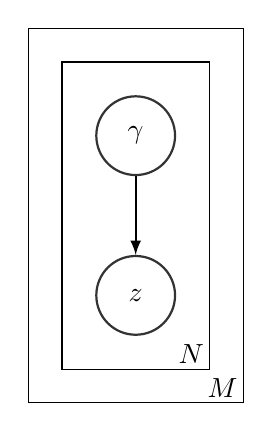
\begin{tikzpicture}
      \tikzstyle{main}=[circle, minimum size = 10mm, thick, draw =black!80, node distance = 10mm]
      \tikzstyle{observed}=[circle, minimum size = 10mm, thick, draw=black!80, node distance = 10mm, fill = black!10]
      \tikzstyle{invismain}=[circle, minimum size = 10mm, thick, draw =white!100, node distance = 10mm]
      \tikzstyle{connect}=[-latex, thick]
      \tikzstyle{box}=[rectangle, draw=black!100, inner sep=12pt]
      \tikzstyle{lbl}=[anchor=south east, inner sep=2pt];

      \node[main] (gamma) {$\gamma$};
      \node[main] (z) [below=of gamma] {$z$};

      \path (gamma) edge [connect] (z);

      \node[box, fit=(gamma) (z)] (N) {};
      \node[box, fit=(gamma) (z) (N)] (M) {};
      \node[lbl] at (N.south east) {$N$};
      \node[lbl] at (M.south east) {$M$};
    \end{tikzpicture}
  \end{center}
  \caption{Graphical model for the factorized variational distribution for
  collapsed variational bayes~\cite{Teh:2007:CVB}.}
  \label{fig:cvbvardist}
\end{figure}

Minimizing the KL-divergence between their variational distribution $q_j(z)$
and the true (collapsed) posterior $p_j(z)$, they arrive at the following
updating equation for $\hat{q}(z_{m,n} = k \mid \hat{\gamma}_{m,n}) =
\hat{\gamma}_{m,n,k}$ as (letting $w_{m,n} = v$):
\begin{align}
  \hat{\gamma}_{m,n,k} &=
  \frac{\exp\left(E_{\hat{q}(\mathbf{Z}_{\neg m,n})}\left[P(\mathbf{W},
  \mathbf{Z}_{\neg m,n}, z_{m,n} = k \mid \alpha, \beta)\right]\right)}
  {\sum_{i=1}^K \exp\left(E_{\hat{q}(\mathbf{Z}_{\neg m,n})}\left[P(\mathbf{W},
  \mathbf{Z}_{\neg m,n}, z_{m,n} = i \mid \alpha, \beta)\right]\right)}\\
  &= \frac{\exp\left(E_{\hat{q}(\mathbf{Z}_{\neg m,n})}\left[
  \log(\alpha_k + \sigma_{m,k}^{\neg m,n})
  + \log(\beta_v + \delta_{k,v}^{\neg m,n})
  - \log(\sum_{r=1}^V \beta_r + \delta_{k,r}^{\neg m,n})\right]\right)}
  {\sum_{i=1}^K \exp\left(E_{\hat{q}(\mathbf{Z}_{\neg m,n})}\left[
      \log(\alpha_i + \sigma_{m,i}^{\neg m,n})
      + \log(\beta_v + \delta_{i,v}^{i,\neg m,n})
    - \log(\sum_{r=1}^V \beta_r + \delta_{i,r}^{\neg m,n})
  \right]\right)}.
\end{align}

The pain point is in calculating the expectations in the above formula.
While the authors give an exact evaluation, this exact evaluation is
computationally infeasible and thus they appeal to a ``Gaussian
approximation'' for the expectations.

They begin by noticing that $\sigma_{m,k}^{\neg m,n} = \sum_{t \neq n}
\mathbb{1}(z_{m,t} = k)$ is a sum of Bernoulli random variables with a mean
parameter $\hat{\gamma}_{m,t,k}$ and thus can be accurately approximated
with a Gaussian with mean $E_{\hat{q}}[\sigma_{m,k}^{\neg m,n}] =
\sum_{t\neq n} \hat{\gamma}_{m,t,k}$ and variance
$Var_{\hat{q}}[\sigma_{m,k}^{\neg m,n}] = \sum_{t\neq n}
\hat{\gamma}_{m,t,k}(1-\hat{\gamma}_{m,t,k})$. They approximate the
logarithms with a second order Taylor series and evaluate the expectation
under the Gaussian approximation (they argue that their second order
approximation is ``good enough'' because $E_{\hat{q}}[\sigma_{m,k}^{\neg
m,n}] \gg 0$). Using this approximation, the updates for CVB become:
\begin{align}
  \hat{\gamma}_{m,n,k} &\propto
  \left(E_{\hat{q}}[\sigma_{m,k}^{\neg m,n}] + \alpha_k\right)
  \frac{\left(E_{\hat{q}}[\delta_{k,v}^{\neg m,n}] + \beta_v\right)}
  {\left(\sum_{r=1}^V E_{\hat{q}}[\delta_{k,r}^{\neg m,n}] +
  \beta_r\right)}\nonumber\\
  &\quad\quad\;
  \times\exp\left(
    -\frac{Var_{\hat{q}}(\sigma_{m,k}^{\neg m,n})}
    {2\left(\alpha_k + E_{\hat{q}}[\sigma_{m,k}^{\neg m,n}]\right)^2}
    -\frac{Var_{\hat{q}}(\delta_{k,v}^{\neg m,n})}
    {2\left(\beta_v + E_{\hat{q}}[\delta_{k,v}^{\neg m,n}]\right)^2}
    +\frac{Var_{\hat{q}}\left(\sum_{r=1}^V \delta_{k,r}^{\neg m,n}\right)}
    {2\left(\sum_{r=1}^V \beta_r + \delta_{k,r}^{\neg m,n}\right)^2}
  \right)
  \label{eqn:cvb}
\end{align}

The similarity with CGS as given in Equation~\ref{eqn:cgs} is apparent. In
particular, the first term is just CGS with the counts $\sigma$ and
$\delta$ replaced with their expectations with respect to the variational
distribution $\hat{q}(\bullet)$, and the second term can be interpreted as
``correction factors'' accounting for the variance~\cite{Teh:2007:CVB}.

The distributions of interest, $\Theta$ and $\Phi$, can be extracted using
a similar method to that used in CGS, but by using the expectations of the
counts with respect to $\hat{q}(\bullet)$ instead of the counts directly.
Namely,
\begin{align}
  \theta_{j,k}
  &\approx
  \frac{(E_{\hat{q}}[\sigma_{j,k}] + \alpha_k)}
  {\left(\sum_{i=1}^K E_{\hat{q}}[\sigma_{j,i}] + \alpha_i\right)}\\
  \phi_{k,v}
  &\approx
  \frac{(E_{\hat{q}}[\delta_{k,v}] + \beta_v)}
  {\left(\sum_{r=1}^V E_{\hat{q}}[\delta_{k,r}] + \beta_r\right)}.
\end{align}

\subsubsection{Evaluation and Implementation Concerns}

While the authors proved that CVB has a better posterior approximation as
compared to the variational Bayes (VB) inference of \citet{Blei:2003:LDA},
they also provided some empirical results to justify their method.

To evaluate just how much better the CVB approximation was when
compared to VB, they looked at the variational bounds for VB vs CVB at
different numbers of iterations. As expected, the variational bound for CVB
was strictly better than VB across all iterations for both datasets they
investigated. They also ran both algorithms to convergence several times
and looked at the distributions of the variational bounds generated by both
algorithms, finding that CVB consistently outperformed VB as to be
expected.

To see how close to the real posterior their CVB approximation got, they
compared CVB to CGS in terms of test set word log probabilities for
different numbers of iterations. The findings were mixed: on one dataset
their method converged in approximately 30 iterations, but CGS surpassed it
at about 25 iterations and continued to get better results as far as 100
iterations. In the other dataset, their algorithm converged in
approximately 20 iterations and was only surpassed by CGS at approximately
40 iterations. In general, it appears that CGS will converge to a strictly
better approximation of the posterior, but this is expected as it
asymptotically should approach the real posterior. CVB has the potential to
converge faster than either CGS and VB.

CVB may be implemented by keeping track of the mean and variance of the
counts $\sigma$ and $\delta$ with respect to $\hat{q}(\bullet)$, and lacks
the repeated calls to the $\Psi(\bullet)$ function that plague standard VB.
Furthermore, they can store only one copy of the variational parameter for
every unique document-word pair $(j,r)$ and have the same memory
requirements as VB. The authors claim that CVB performs less operations per
iteration than CGS, but that the constants for CGS are smaller. However, as
we will see in the next section, the operations per iteration can be
dropped even further by using a simpler approximation.

%What is missing from their evaluation results is a raw speed comparison:
%how much faster does CVB converge to an acceptable threshold compared to
%CGS? Because the number of operations per iteration is different, it is
%potentially unfair to benchmark them on a time scale that is in terms of
%iterations and not in terms of actual wall-clock time. It is a useful
%empirical result to discover that CVB is faster at achieving some threshold
%than CGS for application development where time may be critical.  This can
%be sort-of inferred from the slope in their graphs, but an actual
%experiment surrounding this would have been nice.

\subsection{Lower-order Approximations}
\citet{Asuncion:2009:onsmoothing} propose an alternative method for setting
$\hat{\gamma}_{m,n,k}$ that uses only the zeroth-order information instead
of the second-order information used in Equation~\ref{eqn:cvb}. Namely,

\begin{equation}
  \hat{\gamma}_{m,n,k} \propto
  \left(E_{\hat{q}}[\sigma_{m,k}^{\neg m,n}] + \alpha_k\right)
  \frac{\left(E_{\hat{q}}[\delta_{k,v}^{\neg m,n}] + \beta_v\right)}
  {\left(\sum_{r=1}^V E_{\hat{q}}[\delta_{k,r}^{\neg m,n}] +
  \beta_r\right)}.
  \label{eqn:cvb0}
\end{equation}

They refer to this algorithm as CVB0, and note its extreme similarity to
CGS's sampling in Equation~\ref{eqn:cgs}. The only difference between these
two algorithms is that CGS maintains a topic assignment $z_{m,n}$ for each
token in each document, while CVB0 maintains a distribution over topic
assignments for each token $(m,n)$.

\subsubsection{Evaluation and Implementation Concerns}
CVB0 can be implemented in a very similar way to CVB, except that
statistics for the variance terms need not be calculated. The authors
propose that their algorithm is more performant than CVB for this
reason---lack of variance statistics and calls to $\exp(\bullet)$ should
make the iterations faster.

They evaluate their results in this respect by comparing how long it takes,
in seconds, for each algorithm to reach a certain perplexity level on the
training data. The table is replicated here as Table~\ref{table:cvb0time}.
The find that, across all three of their datasets, CVB0 converges faster or
as fast as CGS. This makes intuitive sense: CVB0 is essentially CGS but
with propagation of uncertainty throughout the sampling process. The
authors also provide results for a parallelized version of CVB0, which
(while little detail was given) is very likely to be similar to the work
for AD-LDA in \citet{Newman:2009:ADLDA}. We call it ``AD-CVB0'' here.

\begin{table}[h]
  \begin{center}
    \begin{tabular}{l|r|r|r}
      & \textbf{MED} & \textbf{KOS} & \textbf{NIPS}\\\hline
      VB & 151.6 & 73.8 & 126.0\\
      CVB & 25.1 & 9.0 & 21.7\\
      CGS & 18.2 & 3.8 & 12.0\\
      CVB0 & 9.5 & 4.0 & 8.4\\
      AD-CVB0 & 2.4 & 1.5 & 3.0\\
    \end{tabular}
  \end{center}
  \caption{Timing results, in seconds, for the different inference algorithms discussed
    so far to reach a fixed perplexity threshold set
    in \citet{Asuncion:2009:onsmoothing}}
  \label{table:cvb0time}
\end{table}

%This is the experiment I was looking for from \citet{Teh:2007:CVB}, but it
%would have been nice to see a bit more results here. For instance, what is
%the variance in these running times? One would expect CGS to have a higher
%variance in running times due to the non-deterministic sampling algorithm,
%but little information is available in the paper on this. Further, are
%these time differences statistically significant? In particular, can we say
%that CVB0 is statistically significantly faster than CGS at reaching a
%fixed perplexity threshold? These questions remain unanswered by this
%simplistic table.

\section{An Aside: Analogy to $k$-means vs EM Clustering}

Consider for a moment the task of clustering tokens into $K$ distinct
clusters. Two general approaches exist: one is to suggest that each
individual token belongs to a single cluster and perform a ``hard
assignment'' of that token to a cluster. This has an advantage that it's
easy to understand, but a disadvantage in that it loses out on the
uncertainty that comes with that cluster assignment. Instead, we could
choose to do a ``soft assignment'' of the token to the clusters, where the
cluster assignment for each token $n$ can be viewed as a vector of
probabilities $v_n$ that, when indexed by a cluster id $k$, yields
$v_{n,k} = P(z_n = k)$, the probability of membership to that cluster.

CGS performs the first option, where each draw from Equation~\ref{eqn:cgs}
assigns a distinct topic to the $n$-th token in document $m$, where as CVB
(and, by extension, CVB0) performs the second option where ``cluster
membership'' is ``topic membership'' and is indexed by
$\hat{\gamma}_{m,n,k}$. Thus, it is interesting to think about CGS as a
``hard assignment'' token clustering algorithm and CVB(0) as a ``soft
assignment'' clustering algorithm.

\section{Online (Stochastic) Methods for Inference in LDA}

Every method discussed thus far has been a \emph{batch learning} method:
take each of the documents in $D$ and update your model parameters by
cycling through every document $d_j \in D$. It is well established in the
machine learning community that \emph{stochastic} optimization algorithms
often outperform batch optimization algorithms. For example, SGD has been
shown to significantly outperform L-BFGS for the task of learning
conditional random
fields\footnote{\url{http://leon.bottou.org/projects/sgd}}.

Because the sizes of our text corpora are always growing, it would be
incredibly beneficial for us to be able to learn our topic models in an
online fashion: treat each document as it is arriving as sampled uniformly
at random from the set of all possible documents, and perform inference
using just this one example (or a small set of examples in mini-batch
setup). In this section, we will explore two new stochastic algorithms for
inference in LDA models: stochastic variational
inference~\cite{Hoffman:2013:svb} and stochastic collapsed variational
inference~\cite{Foulds:2013:scvb}.

\subsection{Stochastic Variational Inference}
Stochastic variational inference~\cite{Hoffman:2013:svb} for LDA is a
modification of the variational Bayes inference algorithm presented
in \citet{Blei:2003:LDA} to an online setting. They present it in a general
form as follows: first, separate the variables of the variational
distribution into a set of ``local'' and ``global'' variables. The
``local'' variables should be specific to a data point, and the ``global''
variables are in some form an aggregation over all of the data points. The
algorithm then proceeds as given in Algorithm~\ref{alg:svi}.

\begin{algorithm}
  \begin{algorithmic}
    \State Initialize the global parameters randomly,

    \State Set a step schedule $\rho_t$ appropriately,

    \Repeat

      Sample data point $x_i$ from the data set uniformly,

      Compute local parameters,

      Compute intermediate global parameters as if $x_i$ was replicated $N$
      times,

      Update the current estimate of global parameters according to the
      step schedule $\rho_t$.
    \Until{termination criterion met}
  \end{algorithmic}
  \caption{Stochastic Variational Inference}
  \label{alg:svi}
\end{algorithm}


(As a refresher, refer to Figure~\ref{fig:factdistsmooth} for the
variational parameter definitions.) They begin by separating the
variational distribution parameters into the ``global'' and ``local''
parameters. For LDA, the global parameters are the topics $\lambda_{i}$,
and the local parameters are document-specific topic proportions $\gamma_j$
and the token-specific topic assignment distribution parameters $\pi_{j,t}$.

Let $\lambda^{(t)}$ be the topics found after iteration $t$. Then, the
algorithm proceeds as follows: sample a document $j$ from the corpus,
compute its local variational parameters $\gamma_j$ and $\pi_j$ by
iterating between the two just as is done in standard variational
inference.

Once these parameters are found, they are used to find the ``intermediate''
global parameters:

\begin{equation}
\hat{\lambda}_{i,r} = \beta_r + M \sum_{t=1}^{N_j}
\pi_{j,t,i}\mathbb{1}(w_{j,t} = r)
\end{equation}

and then we set the global parameters to be an average of the intermediate
$\hat{\lambda}_i$ and the global $\lambda_i^{(t)}$ from the previous
iteration:

\begin{equation}
  \lambda_{i,r}^{(t+1)} = (1-\rho_t)\lambda_{i,r}^{(t)} +
  \rho_t\hat{\lambda}_{i,r}
\end{equation}

This makes intuitive sense and has a strong resemblance to stochastic
gradient descent. Thus, the usual considerations for setting a learning
rate schedule $\rho_t$ apply. Namely, a schedule that monotonically
decreases towards (but never reaching) zero is preferred. In the paper,
they suggest a learning rate parameterized by $\kappa$ and $\tau$ as
follows:

\begin{equation}
  \rho_t = \frac{1}{(t+\tau)^\kappa}
\end{equation}

though other, equally valid, schedules exist in the literature for
stochastic gradient descent. The algorithm, much like SGD, can also be
modified to use mini-batches instead of sampling a single document at a
time for the global $\lambda$ update.

\subsubsection{Evaluation and Implementation Concerns}

The authors discuss two main implementation concerns: setting the batch
size and learning rate parameters. They run various experiments, measuring
the log probability of at test set, to see the effect of the different
choices for these parameters. As a general rule, they find that \emph{large
learning rates} ($\kappa \approx 0.9$) and \emph{large batch sizes} are
preferred for this method.

Large batch sizes being preferred is an interesting result, which seems to
indicate that the gradient given by sampling a single document is much too
noisy to actually take a step in the right direction. One interesting
question, then, would be to explore the difference this inference method
has over just running the original VB algorithm on large batches of
documents and merging the models together following a learning rate
schedule like $\rho_t$. This would seem to me to be a very na\"ive
approach, but if it is effective then it would appear to be a much more
general result: stochastic \emph{anything} in terms of inference for
graphic models could be implemented using this very simple framework.

\subsection{Stochastic Collapsed Variational Inference}
A natural extension of stochastic variational inference is given by
\citet{Foulds:2013:scvb} that attempts to collapse the variational
distribution just like CVB from \citet{Teh:2007:CVB}. They additionally use
the zeroth-order approximation given in \citet{Asuncion:2009:onsmoothing}
for efficiency. An additional interesting feature of this model is that,
because of the streaming nature of the algorithm, storing $\gamma_{m,n,k}$
is impossible---working around this limitation can dramatically lower the
memory requirements for CVB0.

First, to handle the constraint of not being able to store the
$\gamma_{m,n,k}$, the authors only compute it locally for each token that
the algorithm examines. Because $\gamma_{m,n,k}$ cannot be stored, they
cannot remove the counts for assignment $(m,n)$ from the
Equation~\ref{eqn:cvb0}. Thus, they determine $\gamma_{m,n,k}$ with the
following approximation (denoting $w_{m,n}$ as $v$):
\begin{equation}
  \gamma_{m,n,k} \propto \left(E_{\hat{q}}[\sigma_{m,k}] + \alpha_k\right)
  \frac{\left(E_{\hat{q}}[\delta_{k,v}] + \beta_v\right)}
  {\left(\sum_{r=1}^V E_{\hat{q}}[\delta_{k,r}] + \beta_r\right)}
  \label{eqn:scvb0gamma}
\end{equation}

Once $\gamma_{m,n,k}$ is computed for a given token, it can be used to
update the statistics $E_{\hat{q}}[\sigma_{m,k}]$ and
$E_{\hat{q}}[\delta_{k,v}]$ (though the latter is done only after a minibatch
is completed using aggregated statistics across the whole minibatch). In
particular, the updating equations are
\begin{align}
  E_{\hat{q}}[\sigma_m^k] &=
  (1-\rho_t^{(\sigma)}) E_{\hat{q}}[\sigma_{j,k}] + \rho_t^{(\sigma)} N_j
  \gamma_{j,m,n}
  \label{eqn:scvb0sigma} \\
  E_{\hat{q}}[\delta_r^k] &=
  (1-\rho_t^{(\delta)}) E_{\hat{q}}[\delta_{k,r}] + \rho_t^{(\delta)}
  \hat{\delta}_{k,r}
  \label{eqn:scvb0delta}
\end{align}
where $\rho^{(\sigma)}$ and $\rho^{(\delta)}$ are separate learning schedules for
$\sigma$ and $\delta$, respectively, and $\hat{\delta}$ is the aggregated
statistics for $\delta$ with respect to the current minibatch. The
algorithm pseudocode is given as Algorithm~\ref{alg:scvb0}.

\begin{algorithm}
  \begin{algorithmic}
    \State Randomly initialize $\delta_{i,r}$ and $\sigma_{j,i}$.
    \For {each minibatch $D_b$}
      \State $\hat{\delta}_r^i = 0$
      \For {document $j$ in $D_b$}
        \For {$b \geq 0$ ``burn-in'' phases}
          \For {$t \in [1,\ldots,N_j]$}
            \State Update $\gamma_{j,t,i}$ via Equation~\ref{eqn:scvb0gamma}
            \State Update $\sigma_{j,i}$ via Equation~\ref{eqn:scvb0sigma}
          \EndFor
        \EndFor
        \For {$t \in [1,\ldots,N_j]$}
          \State Update $\gamma_{j,t,i}$ via Equation~\ref{eqn:scvb0gamma}
          \State Update $\sigma_{j,i}$ via Equation~\ref{eqn:scvb0sigma}
          \State $\hat{\delta}_{i, w_{j,t}} \leftarrow \hat{\delta}_{i, w_{j,t}} +
          N\gamma_{j,t,i}$ where $N$ is the total number of tokens in the
          corpus
        \EndFor
        \State Update $\delta_{i,r}$ via Equation~\ref{eqn:scvb0delta}
      \EndFor
    \EndFor
  \end{algorithmic}
  \caption{Stochastic Collapsed Variational Bayes}
  \label{alg:scvb0}
\end{algorithm}

\subsubsection{Evaluation and Implementation Concerns}

To evaluate their algorithm, the authors employed three datasets and again
measured the test-set log likelihood at different intervals. In this paper,
they chose \emph{seconds} instead of iterations, which is a better choice
when comparing methods based on their speed. They compared against SVB with
appropriate priors set for both algorithms (using the shift suggested
by \citet{Asuncion:2009:onsmoothing}). On one dataset (PubMed), they found
that the two algorithms behaved mostly similar after about one hour, with
SCVB0 outperforming before that time. In the other two datasets (New York
Times and Wikipedia), SCVB0 outperformed SVB.

They also performed a user study to evaluate their method in the vein of
the suggestions of \citet{Chang:2009:tealeaves} and found that their
algorithm found better topics with significance level $\alpha = 0.05$ on a
test where the algorithms were run for 5 seconds each, and with the same
significance level on another study where the algorithms were run for a
minute each.

\section{But Does It Matter? (Conclusion)}

Perhaps the most important question that this survey raises is this:
does your choice of inference method matter? In
\citet{Asuncion:2009:onsmoothing}, a systematic look at each of the
learning algorithms presented in this survey is undertaken, with
interesting results that suggest a shift of the hyperparameters in the
uncollapsed VB algorithms by $-0.5$. This insight prompted a more careful
look at the importance of the parameters on the priors in the LDA model for
the different inference methods.

Their findings essentially prove that there is little difference in the
quality of the output of the different inference algorithms if one is
careful with the hyperparameters. First, if using uncollapsed VB, it is
important to apply the shift of $-0.5$ to the hyperparameters. Across the
board, it is also very important to set the hyperparameters correctly, and
they find that simply using Minka's fixed point
iterations~\cite{Minka:2000:fpiter} is not necessarily guaranteed to find you
the most desireable hyperparameter.  Instead, the takeaway point is to perform
grid search to find suitable settings for the hyperparameters (but this may not
always be feasible in practice, so Minka's fixed point iterations are also
reasonable).

When doing both the hyperparameter shifting and hyperparameter learning
(either via Minka's fixed point iterations or grid search), the difference
between the inference algorithms almost vanishes. They verified this across
several different datasets (seven in all). Other studies of the influence
of hyperparametrs on LDA have been undertaken, such as the
\citet*{Wallach:2009:NIPS} study that have produced interesting results on
the importance of the priors on the topic model (namely, that an asymmetric
prior on $\Theta$ and a symmetric prior on $\phi$ seems to perform the
best). It would appear that paying more attention to the parameters of the
model, as opposed the mechanism used to learn it, has the largest impact on
the overall results of the model.

The main takeaway, then, is that given a choice between a set of different
feasible algorithms for approximate posterior inference, \emph{the only
preference one should have is toward the method that takes the least amount
of time} to achieve a reasonable level of performance. In that regard, the
methods based on collapsed variational inference seem to be the most
promising, with CVB0 and SCVB0 providing a batch and stochastic version of
a deterministic and easy to implement algorithm for approximate posterior
inference in LDA.

\small
\bibliographystyle{plainnat}
\bibliography{bib}
\end{document}
